\documentclass{layout/tudelft-aiaa}

%% Additional packages and commands
\renewcommand{\deg}{\si{\degree}\xspace}
\usepackage[newfloat]{minted} % (recommended)
\usepackage{comment}
\usepackage{biblatex}
\addbibresource{article.bib}
% Set global Minted options
\setminted{linenos, autogobble, frame=lines, framesep=2mm}

%% Defining title, author and affiliation
\title{A preCICE-OpenFAST adapter \\ to couple OpenFAST to CFD simulation tools}
\author{Leonard Willeke}
\affil{Delft University of Technology}

%%%%%%%%%%%%%%%%%%%%%%%%%%%%%
%%%%% Begin of document %%%%%
%%%%%%%%%%%%%%%%%%%%%%%%%%%%%

\begin{document}

\AlwaysPagewidth{

\maketitle

%% Abstract

\begin{abstract}
    \noindent  
    \begin{itemize}
    	\item Flow dynamics in wind parks are important for many engineering problems from optimized control to load reduction
    	\item High-fidelity flow computation, eg in OpenFOAM, is desirable to understand the farm flow dynamic
    	\item Low-fidelity simulation of the wind turbines is often sufficient
    	\item OpenFAST allows to simulate one or multiple turbines in low fidelity
    	\item I present a preCICE-OpenFAST adapter to couple OpenFAST to the coupling library preCICE
    	\item preCICE couples simulation programs in a black-box manner to achieve multi-´physics simulations
    	\item The adapter serves as driver code for OpenFAST to steer the simulation and calls preCICE for the data exchange
    	\item As a first proof of concept, a coupling to OpenFOAM with limited capabilities is presented
    \end{itemize}
\end{abstract}

}

%% Nomenclature

\renewcommand{\nompreamble}{\emph{Use this section to provide a list of all symbols used in the report. Provide a concise description. For example:}} %

\printnomenclature[\nomequalsign]

\nomenclature{$A$}{amplitude of oscillation}
\nomenclature{$C_p$}{pressure coefficient}
\nomenclature{$C_x$}{force coefficient in the x direction}
\nomenclature{$C_y$}{force coefficient in the y direction}
\nomenclature{$c$}{chord}
\nomenclature{$dt$}{time step}
\nomenclature{$F_x$}{X component of the resultant pressure force acting on the vehicle}
\nomenclature{$F_y$}{Y component of the resultant pressure force acting on the vehicle}
\nomenclature{$f, g$}{generic functions}
\nomenclature{$h$}{height}
\nomenclature{$i$}{time index during navigation}

%% Main body

\section{Introduction}

\lettrine{T}{his} template is a simple article template following all the guidelines of AE2333-I, based on the official AIAA template. Refer to the AE2333-I Word template to see all the procedures and guidelines. Please note that you are free to use other formatting styles, as long as you are consistent in how you apply them throughout your text. By default, the article is in one column. Switching to two columns can be done using the \emph{twocolumn} global option, resulting in the following first line in article.tex: \emph{\textbackslash documentclass[twocolumn]\{layout/tudelft-aiaa\}}.


\section{Software description}

\subsection{Software components}

\subsubsection{preCICE}
\begin{itemize}
	\item An overview is shown in Figure \ref{fig:precice:overview}
	\item Coupled simulation programs are called \textit{solvers} or \textit{participants}
	\item preCICE connects different solvers to perform a partitioned simulation
	\item preCICE takes care of different coupling aspects such as data mapping and communication
	\item Different coupling schemes can be implemented: Who is coupled o whom, what data is exchanged, which coupling algorithms are used \cite{Gatzhammer:2014}
	\item Multi-coupling: Couple multiple (in theory: arbitrary many) participants in different configurations (explicit, implicit)
	\item Acceleration: Use acceleration algorithms to reach a decent computation time
	\item Time interpolation: Use solvers with different time step sizes
	\item Coupling scheme is defined in the precice-config.xml, the only global file which is accessed by all participants
	\item For each solver, a specific \textit{adapter} is necessary to communicate to preCICE
	\item Adapter is an additional piece of software
	\item Adapter can take many forms depending on the solver, eg.: OpenFOAM - C++ Function object, FEniCS - Python module
	\item Different Language bindings are available: C/C++, Python, Fortran, Julia, Matlab
	\item The Adapter allows the solver to access preCICE and to call the coupling
\end{itemize}

\begin{figure*}[t]
	\centering
	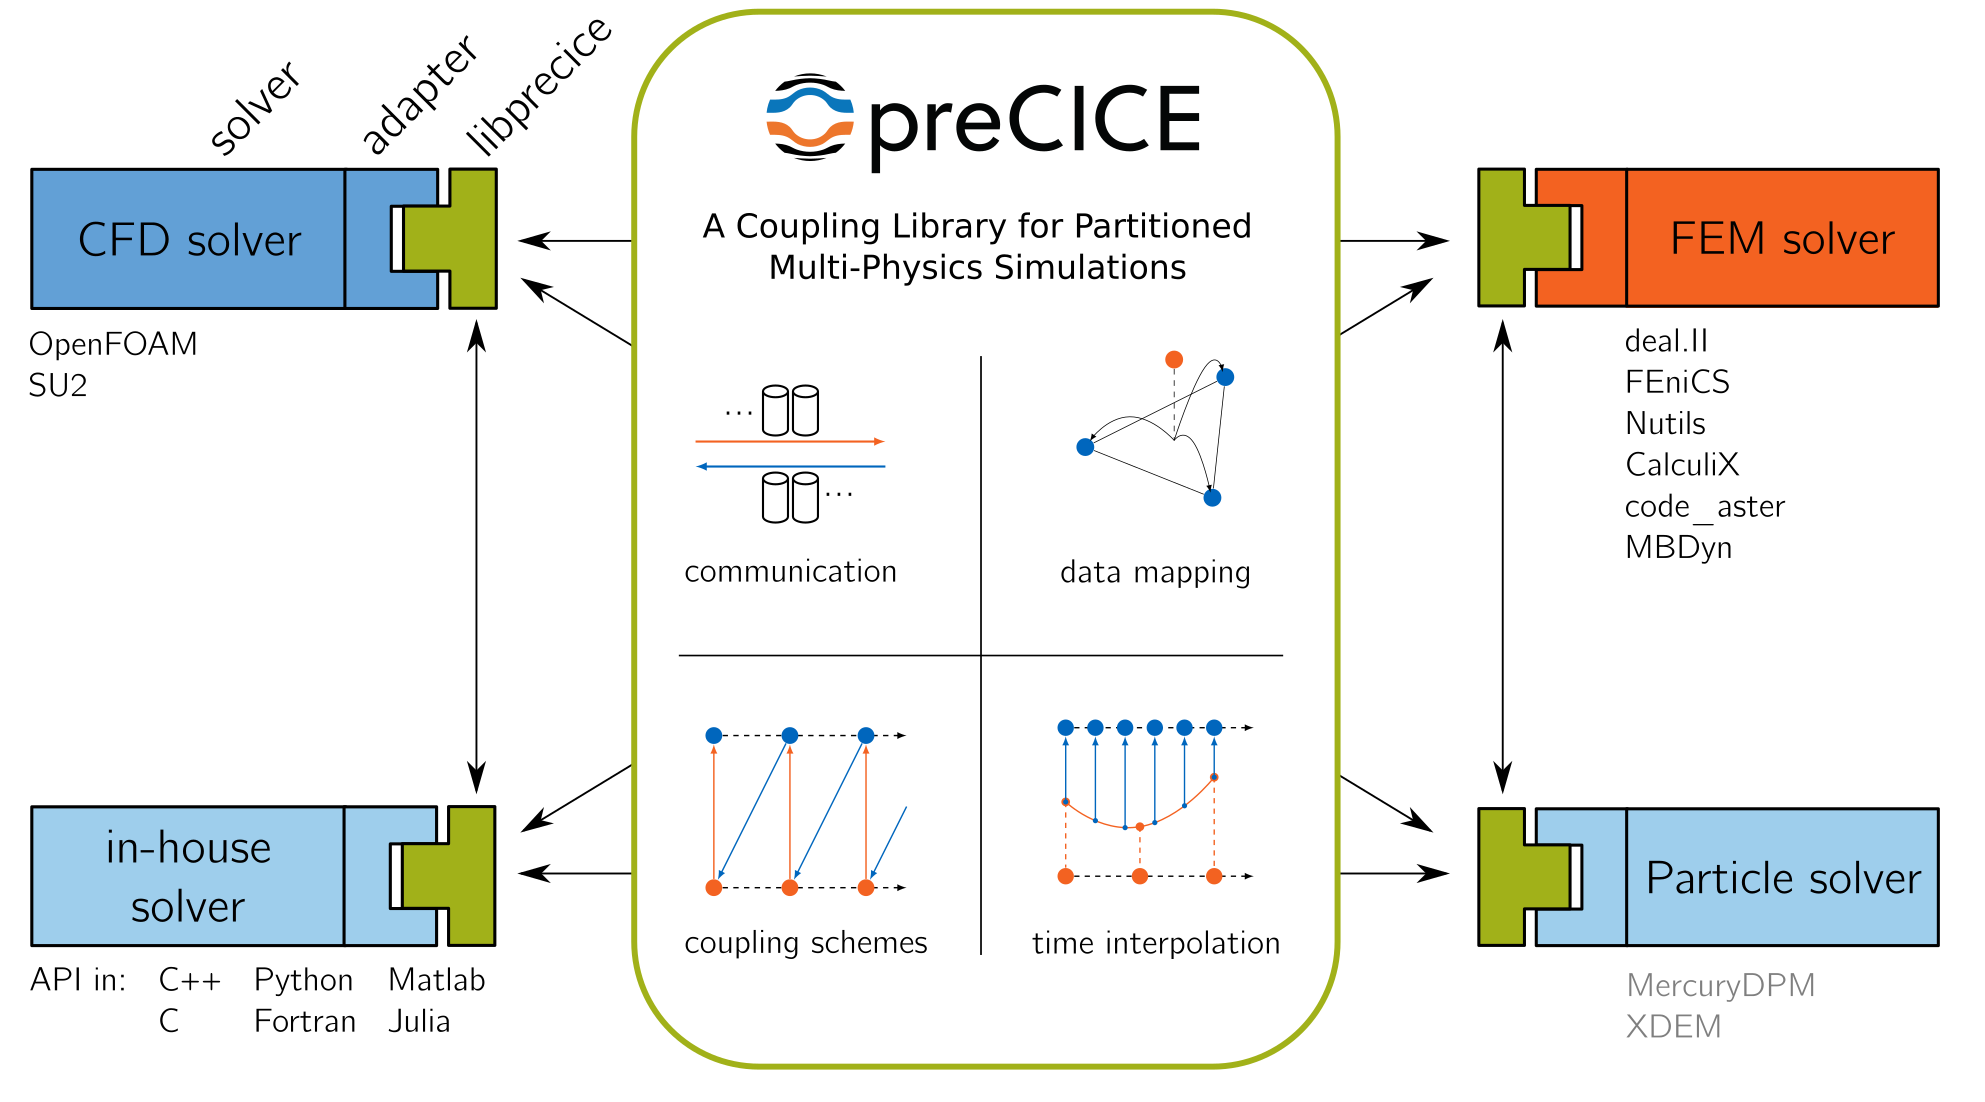
\includegraphics[width=0.9 \textwidth]{images/precice-overview.png}
	\caption{preCICE overview \cite{Chourdakis:2022}}
	\label{fig:precice:overview}
\end{figure*}


\subsubsection{OpenFOAM and the preCICE-OpenFOAM adapter}
\begin{itemize}
	\item OpenFOAM
	\begin{itemize}
		\item Popular open-source PDE tool in academia and industry
		\item Enables the use and modification of different solvers
		\item Used mainly for CFD but also FEM simulations 
	\end{itemize}
	\item Adapter
	\begin{itemize}
		\item Enables the coupling of OpenFOAM via preCICE in different simulation scenarios
		\item Exemplifies the development strategy behind preCICE: Adapter is a library for OpenFOAM and called on runtime to perform the coupling without any modification to the OpenFOAM source code
		\item Different modules for different kinds of multi-physics simulations: FSI, FF, CHT
	\end{itemize}
\end{itemize}	
Note:
I should introduce the OpenFOAM adapter at some point.
Lets introduce the broad concept of the adapter here and add more details, eg about the specific files that would need to be modified, later in the Challenges part
\newline
\subsubsection{OpenFAST}
\begin{itemize}
	\item Wind energy engineering tool developed by NREL
	\item Widely used in academia and industry
	\item Simulates the coupled aerodynamic, structural, and electrical behaviour of wind turbines as well as the control response
	\item Allows to model on- and offshore wind turbines and can be used to compute wind parks as well
	\item OpenFAST is a glue code for different modules which compute the various physical domains
	\item Takes one main input file denoted \textit{.fst} which points to more specific files for each computation module (eg AeroDyn, ServoDyn, ...)
	\item Fidelity: Does OpenFAST include computations in different fidelities? Is it a low- to mid-fidelity tool?
	\item Computes the Fluid-Structure-Interaction at blades and tower with the actuator line method
	\item Inflow field is either computed by AeroDyn or received from external CFD solver
	\item Has a dedicated C++ API for the coupling with CFD solvers
\end{itemize}

OpenFAST is mainly used to perform turbine loads analysis and drive the detailed turbine design. The computational cost is therefore higher than for tools used in the early design exploration phase like WISDEM, RAFT or FLORIS, but lower than highly resolved solvers necessary to understand the actual physics and check the final turbine design like ExaWind or SOWFA. 

\subsection{Software concept}

Main idea
\begin{itemize}
	\item Write a preCICE-OpenFAST adapter (see Figure \ref{fig:setup}), a new piece of software that connects OpenFAST and preCICE
	\item Acts as driver code towards OpenFAST: Calls it via the C++ API
	\item Calls preCICE to communicate data and steering commands
	\item Configurable by two .yaml input files
	\item preciceSettings.yaml contains information about the coupling setup
	\item openfastSettings.yaml contains information about the turbine simulation case
	\item The concept is sketched out in Figure \ref{code:adapter}
	\item line 8-10: Instantiate and initialize the interface to OpenFAST
	\item line 12-14: Do the same for preCICE
	\item Now both software component are ready to use
	\item line 16: main time loop controlled by preCICE
	\item line 18: Read velocity data from CFD solver via preCICE and store it in local variable
	\item line 20: Set the velocity data in OpenFAST
	\item line 22: Tell OpenFAST to compute the wind turbine dynamics for the next time step
	\item line 24: Get the resulting force from OpenFAST and store it in local variable
	\item line 26: Send force data to CFD solver to be used in ALM method
	\item line 28: Advance both solvers in time
	\item line 30-31: End the simulation after the main loop has finished
	\item Developed and documented on GitHub\footnote{\url{https://github.com/LeonardWilleke/openfast-adapter}}\\
\end{itemize}

\begin{comment}
	The OpenFAST adapter is something between the FMI Runner and a normal adapter:
	It executes OpenFAST like the runner but OpenFAST is a full, executable program on
	its own.
	
	\begin{figure*}[t]
	\centering
	\includegraphics[width=0.9 \textwidth]{images/precice-openfast-adapter-setup.png}
	\caption{preCICE-OpenFAST Adapter software architecture}
	\label{fig:openfast:adapter}
	\end{figure*}
\end{comment}


\begin{figure}[h!]
	\centering
	\begin{minipage}{0.9\textwidth}
		\begin{minted}{cpp}
		#include <OpenFAST.H>
		#include <precice.hpp>
		
		vector<double> readData;
		vector<double> writeData;
		
		// OpenFAST Setup
		fast::OpenFAST FAST;
		...
		FAST.init()
		// preCICE Setup
		participant = precice.participant(...);
		...
		participant.initialize();
		// main time loop
		while participant.isCouplingOngoing(): 
			// Get read data from preCICE
			participant.readData(readData, ...);
			// Set read data in OpenFAST
			FAST.setVelocity(readData, ...);
			// Compute next time step
			FAST.step();
			// Get write data from OpenFAST
			FAST.getForce(writeData, ...);
			// Send write data to preCICE
			participant.writeData(writeData, ...);
			// Advance preCICE in time
			participant.advance(dt) 
		
		participant.finalize()
		FAST.end()
		\end{minted}
	\end{minipage}
	\caption{Concept of the OpenFAST adapter: The script utilizes the C++ API to execute OpenFAST and calls preCICE to couple the simulation. For conciseness, API calls are simplified.}
	\label{code:adapter}
\end{figure}


\section{Results \& Discussion}

In some cases, it might be prefered to split this part into two sections.


\section{Challenges}
\label{section:challenges}

What are the next steps in the coupling of OpenFAST via preCICE? This section aims to give an overview of the upcoming tasks to guide interested developers in their endeavour. 

\subsection{Mapping turbine data between actuator lines and volume meshes}

The most pressing issue is to implement a correct mapping. As seen in chapter \ref{section:cases}, the mapping depends not only on the preCICE-OpenFAST adapter, but also on the preCICE adapter of the CFD solver. In our case, we face problems because the OpenFOAM adapter was not designed for the implementation of ALM. In particular, the volume coupling functionalities are not sufficient. It is possible to retrieve velocity data from a volume. But it is not possible to write force or pressure gradient data on a volume. However, this functionality is needed to implement a bidirectional coupling for this FSI case. I see two solutions to this problem:\\
\textbf{Solution 1: Map in the OpenFAST adapter}\\
The code\footnote{\url{https://gitlab.com/whiffle-public/aspfast} (visited on 28.12.2023)} from AspFAST provides a possible solution. The tool to connect OpenFAST and GRASP is published under a MIT license and can therefore be re-used without limitations. It implements useful mapping functions in the main script \textit{aspast.cpp}. To communicate from OpenFAST to the CFD solver, the functions \textit{calcBodyForce}, \textit{uniformBodyForce} and \textit{diskBodyForce} are used. To understand the mapping from CFD to OpenFAST, look into the functions \textit{sampleVelocity} and \textit{calcVelocity}. Including similar functions in the OpenFAST adapter could help to address mapping problems. It is still unclear how the mapped force values would then be transferred to a volume mesh in OpenFOAM.\\[12pt]
\textbf{Solution 2: Modify the OpenFOAM adapter}\\
Another solution is to add the missing functionality in the OpenFOAM adapter. For the coupling setup, the Fluid-Fluid (FF) module of the adapter is used. For a correct coupling, OpenFOAM needs to include the updated field values of force or pressure gradient from OpenFAST. But the OpenFOAM adapter only supports the exchange of pressure as field value. To change this, we need to adapt the class \textit{PressureGradient.C} of the FF module. A code section to write pressure gradient data on a cellset should be added. Have a look in the class \textit{Pressure.C} of the FF module to get an idea how to access and write field values in OpenFOAM in general.

Inside OpenFOAM, the pressure gradient is stored as the boundary condition of the velocity field U. Therefore, we need to import the velocity field U in the class \textit{PressureGradient.C} and use appropriate commands from OpenFOAM to set its boundary condition. Setting the boundary condition on a cellset and not on a wall or inlet might be tricky.

As an additional remark, the OpenFOAM library turbinesFoam\footnote{\url{https://github.com/turbinesFoam/turbinesFoam} (visited 14.12.2023)} \cite{Bachant:2018} might be useful. It implements the actuator line method with different solvers like pimpleFoam. The solvers are modified to perform the ALM computation. It is not clear yet how this could be of use, as we want to perform the ALM computation of the turbine in OpenFAST and map the results to OpenFOAM, not do the whole computation in OpenFOAM.

\begin{comment}

\begin{itemize}
	\item Problem: The OpenFOAM adapter is not designed for the implementation of ALM
	\item We need to get velocity from a volume section --> possible
	\item We need to set force or pressure gradient on a volume section --> not possible
	\item Solution 1: Do the mapping in the OpenFAST adapter
	\begin{itemize}
		\item Something very similar has been done by AspFAST (LINK)
		\item The MIT license of the software allows to re-use it without limitations
		\item What exactly needs to be done?
		\begin{itemize}
			\item Look into aspfast.cpp
			\item Understand how the mapping from OpenFAST to the CFD solver is done in the functions \textit{calcBodyForce}, \textit{uniformBodyForce} and \textit{diskBodyForce}
			\item Understand how the mapping from the CFD solver to OpenFAST works in the functions \textit{sampleVelocity} and \textit{calcVelocity}
		\end{itemize}
		\item Includes smearing of the actuator data which is good
		\item Possible Problem: I add volume data to the mesh in the OpenFAST adapter that the OpenFOAM adapter is not able to write to FOAM afterwards --> think about
	\end{itemize}
	\item Solution 2: Modify the OpenFOAM adapter
		\begin{itemize}
			\item Adapt the PressureGradient.C class of the FF module
			\item Include code to write pressure gradient on a cellset
			\item Take structure from Pressure.C class
			\item Problem: How to write the pressure gradient on a field in OpenFOAM?
			\item Pressure gradient seems to be the boundary condition of the velocity field U --> this is settable
			\item Requires the correct import of the velocity field and the correct retrieval of its boundary field --> give the commands you know
			\item Not sure if you can also set the pressure gradient on the pressure field itself but dont think so
			\item Open: How to do smearing if necessary\\
		\end{itemize}
	\item Additional remark: The OpenFOAM library turbinesFoam\footnote{\url{https://github.com/turbinesFoam/turbinesFoam} (visited 14.12.2023)} \cite{Bachant:2018} might be useful. It implements the actuator line method with different solvers like pimpleFoam in OpenFOAM. The solvers are modified to perform the ALM computation. It is not clear yet how this could be of use, as we want to perform the ALM computation of the turbine to OpenFAST and map the results to OpenFOAM, not do the whole computation in OpenFOAM.
\end{itemize}
\end{comment}

\subsection{Improve code maturity}

To railguard the further development, a regression test should be implemented. The dummy fluid solver from chapter \ref{section:cases:dummy} can be used as a simple coupling participant to check calculations. The preCICE-FMI runner\footnote{\url{https://github.com/precice/fmi-runner/tree/main} (visited on 06.01.2024)} may serve as an example on how to write the test, place it in the GitHub repository and execute it automatically with GitHub workflows.

Once a mature coupling to OpenFOAM is achieved, the coupling should be verified. Previous work \cite{Taschner:2022} provides a benchmark case to cross-verify the coupling of a single NREL 5MW turbine with five other research LES codes.
\begin{comment}
\begin{itemize}
	\item Write a regression test (using the dummy fluid solver)
	\item Create a first test case with documentation
	\item Verify simulation results against simulations done with AspFAST and other tools (\cite{Taschner:2022} gives some benchmark cases)\\
\end{itemize}
\end{comment}

\subsection{Enable coupling with multiple turbines}

A future version of the adapter may include the coupling of multiple turbines in OpenFAST with one OpenFOAM instance. The OpenFAST C++ API allows to run multiple instances of OpenFAST to simulate wind park scenarios with FAST.FARM. But how do you communicate the results of multiple turbines to preCICE, and how do you organize the coupling to the CFD solver? This scenario increases the complexity in both adapters involved in the coupling setup. Again, a look into the AspFAST code could provide insight into how to deal with those challenges.

A different option may be the use of the preCICE Micro manager\footnote{\url{https://precice.org/tooling-micro-manager-overview.html} (visited on 06.01.2024)}. It is a tool to manage many micro simulations and couple them to one macro simulation. However, it must be said that the manager was not designed with large-scale FSI simulations in mind.
\begin{comment}
\begin{itemize}
	\item OpenFAST C++ API allows to run multiple instances of OpenFAST for wind park scenarios
	\item How do you connect them to preCICE? 
	\item How do you define the different coupling scenarios?
	\item Possibly use the MacroMicro manager of preCICE to deal with the coupling of multiple domains\\
\end{itemize}
\end{comment}


\subsection{Explore coupling scenarios with other CFD solver}

The current work is focused on the coupling of OpenFAST with OpenFOAM for the simple fact that it is the only suitable CFD solver in the preCICE ecosystem. The coupling of other tools like GRASP, NaluWind or YALES2 via preCICE might be interesting to create a simulation environment where CFD solvers could be swapped easily. Simulation results could be compared mor readily and the individual strengths of each program leveraged depending on the simulation case. However, this setup comes with the additional effort of developing preCICE adapters for the other CFD programs. As the tools above are already coupled to OpenFAST with mature, verified tools, this should only be done if it adds real benefit to the research community.

\begin{comment}
\begin{itemize}
\item Are there currently other CFD solvers coupled to preCICE that would be interesting?
\item Otherwise interesting candidates are: YALES2, GRASP, NaluWind
\item Most of them have native coupling tools for OpenFAST already\\
\end{itemize}

Additional remarks
\begin{itemize}
	\item The OpenFOAM library turbinesFoam\footnote{\url{https://github.com/turbinesFoam/turbinesFoam} (visited 14.12.2023)} \cite{Bachant:2018} might be useful. It implements the actuator line method with different solvers like pimpleFoam in OpenFOAM. The solvers are modified to perform the ALM computation. It is not clear yet how this could be of use, as we want to perform the ALM computation of the turbine to OpenFAST and map the results to OpenFOAM, not do the whole computation in OpenFOAM.
\end{itemize}
\end{comment}


\section{Conclusion}
\label{section:conclusion}

\begin{itemize}
	\item First coupling of OpenFAST and preCICE was presented
	\item Coupling with a dummy solver and OpenFOAM was discussed
	\item Although a proof of concept was achieved, some challenging tasks remain to enable a full coupling to CFD solvers
	\item How to map between OpenFAST and an arbitrary CFD solver? Where to place the mapping and smearing algorithm for the ALM method?
	\item This work may serve as a starting point
	\item Has the potential to be developed into a viable open-source alternative for the coupling of OpenFAST to different CFD solvers
\end{itemize}


\section*{Acknowledgments}

I am grateful to Prof. Axelle Viré who accepted me as a visiting researcher and made this work possible. Many thanks to her and Evert Ewald for the discussions and hints during our meetings. Extended thanks to Benjamin Uekermann, who enabled my visit at TU Delft in the first place and provided feedback along the way. Lastly, I want to thank the wonderful crowd of PhD researchers in the wind energy department who made my time in Delft memorable.

%% Bibliography

\printbibliography

%% Appendix

\section*{Appendix}

Possible points to include in the Appendix
\begin{itemize}
	\item Files from the OpenFOAM adapter with hints on how to modify them
	\item Files from AspFAST with hints on how to reuse the code for our mapping
\end{itemize}

\end{document}
